\documentclass[tikz,border=0mm]{standalone}
\usepackage[utf8]{inputenc}
\usepackage{unicode-math} % for unicode support in math environments
\usepackage{amsmath}
\usepackage{siunitx}
\usepackage{booktabs}
\sisetup{mode=text,range-phrase = {\text{~to~}}, range-units=single, print-unity-mantissa=false}
\usepackage{mhchem}
\usepackage{tikz}



\usepackage{fontspec}

\directlua{
  luaotfload.add_fallback(
  "FallbackFonts",
  {
        "DejaVu Serif:mode=harf;",
        "DejaVu Sans Mono:mode=harf;",
        % we could add many more fonts here optionally!
    }
  )
}

\setmainfont{STIXTwoText}[RawFeature={fallback=FallbackFonts}]
\setmathfont{STIXTwoMath-Regular}[RawFeature={fallback=FallbackFonts}]
\setmonofont{Inconsolata}[RawFeature={fallback=FallbackFonts}]

\begin{document}
\definecolor{backgroundColor}{rgb}{1.0, 1.0, 1.0}

\pagecolor{backgroundColor}


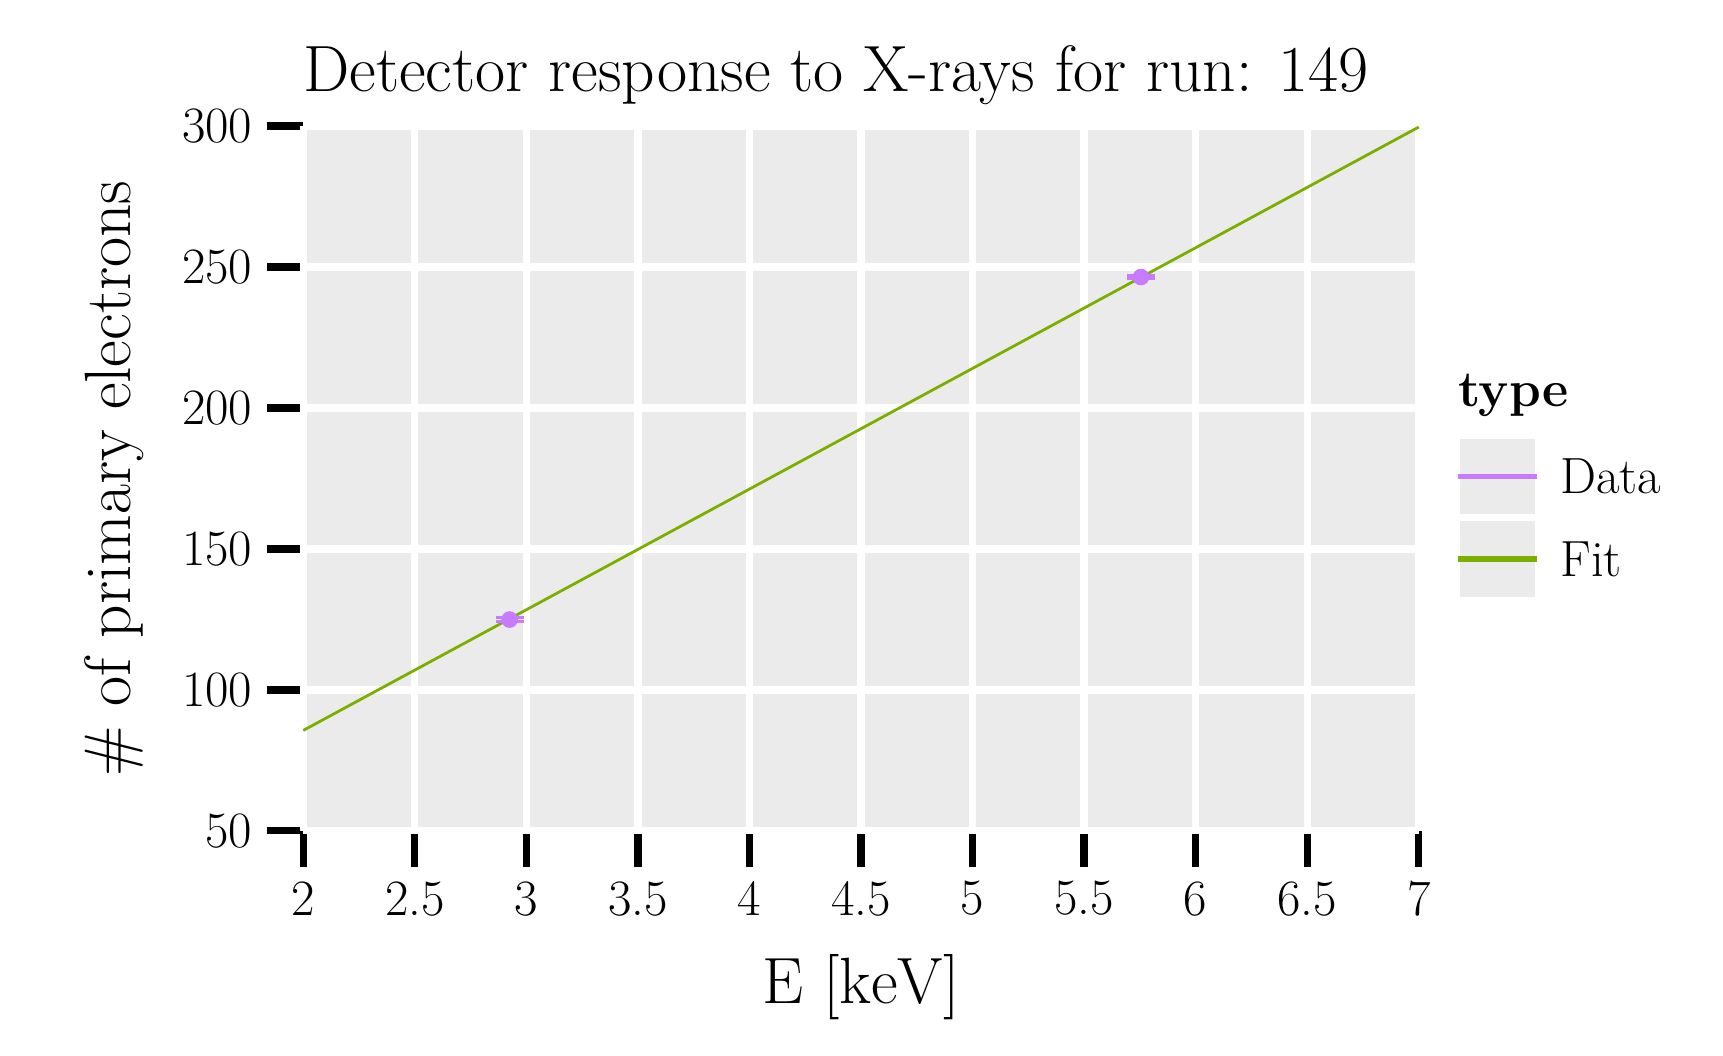
\begin{tikzpicture}[every node/.style={outer sep=0pt, inner sep=0pt}]
\path[use as bounding box] (0, 0) rectangle (600.0bp, 360.0bp) ;
\definecolor{drawColor}{rgb}{0.0, 0.0, 0.0}
\definecolor{fillColor}{rgb}{1.0, 1.0, 1.0}

\draw [color = drawColor, fill = fillColor, draw opacity = 0.0, fill opacity = 1.0, line width = 0.0bp] (0.0000bp, 360.0000bp) rectangle (600.0000bp, 0.0000bp) ;
\node [right, font=\fontsize{23.65409807549184}{28.38491769059021}\selectfont
, anchor=west] at (99.2126bp, 342.9352bp){Detector response to X-rays for run: 149} ;
\definecolor{drawColor}{rgb}{0.0, 0.0, 0.0}
\definecolor{fillColor}{rgb}{0.9200000166893005, 0.9200000166893005, 0.9200000166893005}

\draw [color = drawColor, fill = fillColor, draw opacity = 0.0, fill opacity = 1.0, line width = 0.0bp] (99.2126bp, 324.5669bp) rectangle (500.7874bp, 70.8661bp) ;
\definecolor{drawColor}{rgb}{0.0, 0.0, 0.0}
\definecolor{fillColor}{rgb}{0.0, 0.0, 0.0}

\draw [color = drawColor, fill = fillColor, draw opacity = 1.0, fill opacity = 0.0, line width = 2.628233119499094bp] (99.2126bp, 57.7250bp)--(99.2126bp, 70.8661bp) ;
\draw [color = drawColor, fill = fillColor, draw opacity = 1.0, fill opacity = 0.0, line width = 2.628233119499094bp] (139.3701bp, 57.7250bp)--(139.3701bp, 70.8661bp) ;
\draw [color = drawColor, fill = fillColor, draw opacity = 1.0, fill opacity = 0.0, line width = 2.628233119499094bp] (179.5276bp, 57.7250bp)--(179.5276bp, 70.8661bp) ;
\draw [color = drawColor, fill = fillColor, draw opacity = 1.0, fill opacity = 0.0, line width = 2.628233119499094bp] (219.6850bp, 57.7250bp)--(219.6850bp, 70.8661bp) ;
\draw [color = drawColor, fill = fillColor, draw opacity = 1.0, fill opacity = 0.0, line width = 2.628233119499094bp] (259.8425bp, 57.7250bp)--(259.8425bp, 70.8661bp) ;
\draw [color = drawColor, fill = fillColor, draw opacity = 1.0, fill opacity = 0.0, line width = 2.628233119499094bp] (300.0000bp, 57.7250bp)--(300.0000bp, 70.8661bp) ;
\draw [color = drawColor, fill = fillColor, draw opacity = 1.0, fill opacity = 0.0, line width = 2.628233119499094bp] (340.1575bp, 57.7250bp)--(340.1575bp, 70.8661bp) ;
\draw [color = drawColor, fill = fillColor, draw opacity = 1.0, fill opacity = 0.0, line width = 2.628233119499094bp] (380.3150bp, 57.7250bp)--(380.3150bp, 70.8661bp) ;
\draw [color = drawColor, fill = fillColor, draw opacity = 1.0, fill opacity = 0.0, line width = 2.628233119499094bp] (420.4724bp, 57.7250bp)--(420.4724bp, 70.8661bp) ;
\draw [color = drawColor, fill = fillColor, draw opacity = 1.0, fill opacity = 0.0, line width = 2.628233119499094bp] (460.6299bp, 57.7250bp)--(460.6299bp, 70.8661bp) ;
\draw [color = drawColor, fill = fillColor, draw opacity = 1.0, fill opacity = 0.0, line width = 2.628233119499094bp] (500.7874bp, 57.7250bp)--(500.7874bp, 70.8661bp) ;
\node [font=\fontsize{18.39763183649366}{22.07715820379239}\selectfont
] at (99.2126bp, 46.5549bp){2} ;
\node [font=\fontsize{18.39763183649366}{22.07715820379239}\selectfont
] at (139.3701bp, 46.4348bp){2.5} ;
\node [font=\fontsize{18.39763183649366}{22.07715820379239}\selectfont
] at (179.5276bp, 46.4348bp){3} ;
\node [font=\fontsize{18.39763183649366}{22.07715820379239}\selectfont
] at (219.6850bp, 46.4348bp){3.5} ;
\node [font=\fontsize{18.39763183649366}{22.07715820379239}\selectfont
] at (259.8425bp, 46.5456bp){4} ;
\node [font=\fontsize{18.39763183649366}{22.07715820379239}\selectfont
] at (300.0000bp, 46.4256bp){4.5} ;
\node [font=\fontsize{18.39763183649366}{22.07715820379239}\selectfont
] at (340.1575bp, 46.5641bp){5} ;
\node [font=\fontsize{18.39763183649366}{22.07715820379239}\selectfont
] at (380.3150bp, 46.5641bp){5.5} ;
\node [font=\fontsize{18.39763183649366}{22.07715820379239}\selectfont
] at (420.4724bp, 46.4256bp){6} ;
\node [font=\fontsize{18.39763183649366}{22.07715820379239}\selectfont
] at (460.6299bp, 46.4164bp){6.5} ;
\node [font=\fontsize{18.39763183649366}{22.07715820379239}\selectfont
] at (500.7874bp, 46.6103bp){7} ;
\draw [color = drawColor, fill = fillColor, draw opacity = 1.0, fill opacity = 0.0, line width = 2.628233119499094bp] (99.2126bp, 70.8661bp)--(86.0714bp, 70.8661bp) ;
\draw [color = drawColor, fill = fillColor, draw opacity = 1.0, fill opacity = 0.0, line width = 2.628233119499094bp] (99.2126bp, 121.6063bp)--(86.0714bp, 121.6063bp) ;
\draw [color = drawColor, fill = fillColor, draw opacity = 1.0, fill opacity = 0.0, line width = 2.628233119499094bp] (99.2126bp, 172.3465bp)--(86.0714bp, 172.3465bp) ;
\draw [color = drawColor, fill = fillColor, draw opacity = 1.0, fill opacity = 0.0, line width = 2.628233119499094bp] (99.2126bp, 223.0866bp)--(86.0714bp, 223.0866bp) ;
\draw [color = drawColor, fill = fillColor, draw opacity = 1.0, fill opacity = 0.0, line width = 2.628233119499094bp] (99.2126bp, 273.8268bp)--(86.0714bp, 273.8268bp) ;
\draw [color = drawColor, fill = fillColor, draw opacity = 1.0, fill opacity = 0.0, line width = 2.628233119499094bp] (99.2126bp, 324.5669bp)--(86.0714bp, 324.5669bp) ;
\node [left, font=\fontsize{18.39763183649366}{22.07715820379239}\selectfont
, anchor=east] at (80.8476bp, 70.8661bp){50} ;
\node [left, font=\fontsize{18.39763183649366}{22.07715820379239}\selectfont
, anchor=east] at (80.8476bp, 121.6063bp){100} ;
\node [left, font=\fontsize{18.39763183649366}{22.07715820379239}\selectfont
, anchor=east] at (80.8476bp, 172.3465bp){150} ;
\node [left, font=\fontsize{18.39763183649366}{22.07715820379239}\selectfont
, anchor=east] at (80.8476bp, 223.0866bp){200} ;
\node [left, font=\fontsize{18.39763183649366}{22.07715820379239}\selectfont
, anchor=east] at (80.8476bp, 273.8268bp){250} ;
\node [left, font=\fontsize{18.39763183649366}{22.07715820379239}\selectfont
, anchor=east] at (80.8476bp, 324.5669bp){300} ;
\node [font=\fontsize{23.65409807549184}{28.38491769059021}\selectfont
] at (300.0000bp, 14.6691bp){E [$\si{keV}$]} ;
\node [rotate = 90.0, font=\fontsize{23.65409807549184}{28.38491769059021}\selectfont
] at (31.1560bp, 197.7165bp){\# of primary electrons} ;
\definecolor{drawColor}{rgb}{1.0, 1.0, 1.0}
\definecolor{fillColor}{rgb}{0.0, 0.0, 0.0}

\draw [color = drawColor, fill = fillColor, draw opacity = 1.0, fill opacity = 0.0, line width = 2.628233119499094bp] (99.2126bp, 324.5669bp)--(99.2126bp, 70.8661bp) ;
\draw [color = drawColor, fill = fillColor, draw opacity = 1.0, fill opacity = 0.0, line width = 2.628233119499094bp] (139.3701bp, 324.5669bp)--(139.3701bp, 70.8661bp) ;
\draw [color = drawColor, fill = fillColor, draw opacity = 1.0, fill opacity = 0.0, line width = 2.628233119499094bp] (179.5276bp, 324.5669bp)--(179.5276bp, 70.8661bp) ;
\draw [color = drawColor, fill = fillColor, draw opacity = 1.0, fill opacity = 0.0, line width = 2.628233119499094bp] (219.6850bp, 324.5669bp)--(219.6850bp, 70.8661bp) ;
\draw [color = drawColor, fill = fillColor, draw opacity = 1.0, fill opacity = 0.0, line width = 2.628233119499094bp] (259.8425bp, 324.5669bp)--(259.8425bp, 70.8661bp) ;
\draw [color = drawColor, fill = fillColor, draw opacity = 1.0, fill opacity = 0.0, line width = 2.628233119499094bp] (300.0000bp, 324.5669bp)--(300.0000bp, 70.8661bp) ;
\draw [color = drawColor, fill = fillColor, draw opacity = 1.0, fill opacity = 0.0, line width = 2.628233119499094bp] (340.1575bp, 324.5669bp)--(340.1575bp, 70.8661bp) ;
\draw [color = drawColor, fill = fillColor, draw opacity = 1.0, fill opacity = 0.0, line width = 2.628233119499094bp] (380.3150bp, 324.5669bp)--(380.3150bp, 70.8661bp) ;
\draw [color = drawColor, fill = fillColor, draw opacity = 1.0, fill opacity = 0.0, line width = 2.628233119499094bp] (420.4724bp, 324.5669bp)--(420.4724bp, 70.8661bp) ;
\draw [color = drawColor, fill = fillColor, draw opacity = 1.0, fill opacity = 0.0, line width = 2.628233119499094bp] (460.6299bp, 324.5669bp)--(460.6299bp, 70.8661bp) ;
\draw [color = drawColor, fill = fillColor, draw opacity = 1.0, fill opacity = 0.0, line width = 2.628233119499094bp] (500.7874bp, 324.5669bp)--(500.7874bp, 70.8661bp) ;
\draw [color = drawColor, fill = fillColor, draw opacity = 1.0, fill opacity = 0.0, line width = 2.628233119499094bp] (99.2126bp, 70.8661bp)--(500.7874bp, 70.8661bp) ;
\draw [color = drawColor, fill = fillColor, draw opacity = 1.0, fill opacity = 0.0, line width = 2.628233119499094bp] (99.2126bp, 121.6063bp)--(500.7874bp, 121.6063bp) ;
\draw [color = drawColor, fill = fillColor, draw opacity = 1.0, fill opacity = 0.0, line width = 2.628233119499094bp] (99.2126bp, 172.3465bp)--(500.7874bp, 172.3465bp) ;
\draw [color = drawColor, fill = fillColor, draw opacity = 1.0, fill opacity = 0.0, line width = 2.628233119499094bp] (99.2126bp, 223.0866bp)--(500.7874bp, 223.0866bp) ;
\draw [color = drawColor, fill = fillColor, draw opacity = 1.0, fill opacity = 0.0, line width = 2.628233119499094bp] (99.2126bp, 273.8268bp)--(500.7874bp, 273.8268bp) ;
\draw [color = drawColor, fill = fillColor, draw opacity = 1.0, fill opacity = 0.0, line width = 2.628233119499094bp] (99.2126bp, 324.5669bp)--(500.7874bp, 324.5669bp) ;
\definecolor{drawColor}{rgb}{0.4848798215389252, 0.683388352394104, 0.0}
\definecolor{fillColor}{rgb}{0.0, 0.0, 0.0}

\draw [color = drawColor, fill = fillColor, draw opacity = 1.0, fill opacity = 0.0, line width = 1.0bp]
(99.2126bp, 107.0098bp)  -- 
(103.2689bp, 109.2038bp)  -- 
(107.3252bp, 111.3978bp)  -- 
(111.3815bp, 113.5919bp)  -- 
(115.4378bp, 115.7859bp)  -- 
(119.4942bp, 117.9800bp)  -- 
(123.5505bp, 120.1740bp)  -- 
(127.6068bp, 122.3680bp)  -- 
(131.6631bp, 124.5621bp)  -- 
(135.7194bp, 126.7561bp)  -- 
(139.7757bp, 128.9501bp)  -- 
(143.8320bp, 131.1442bp)  -- 
(147.8883bp, 133.3382bp)  -- 
(151.9446bp, 135.5322bp)  -- 
(156.0010bp, 137.7263bp)  -- 
(160.0573bp, 139.9203bp)  -- 
(164.1136bp, 142.1143bp)  -- 
(168.1699bp, 144.3084bp)  -- 
(172.2262bp, 146.5024bp)  -- 
(176.2825bp, 148.6964bp)  -- 
(180.3388bp, 150.8905bp)  -- 
(184.3951bp, 153.0845bp)  -- 
(188.4514bp, 155.2786bp)  -- 
(192.5078bp, 157.4726bp)  -- 
(196.5641bp, 159.6666bp)  -- 
(200.6204bp, 161.8607bp)  -- 
(204.6767bp, 164.0547bp)  -- 
(208.7330bp, 166.2487bp)  -- 
(212.7893bp, 168.4428bp)  -- 
(216.8456bp, 170.6368bp)  -- 
(220.9019bp, 172.8308bp)  -- 
(224.9582bp, 175.0249bp)  -- 
(229.0146bp, 177.2189bp)  -- 
(233.0709bp, 179.4129bp)  -- 
(237.1272bp, 181.6070bp)  -- 
(241.1835bp, 183.8010bp)  -- 
(245.2398bp, 185.9950bp)  -- 
(249.2961bp, 188.1891bp)  -- 
(253.3524bp, 190.3831bp)  -- 
(257.4087bp, 192.5771bp)  -- 
(261.4650bp, 194.7712bp)  -- 
(265.5214bp, 196.9652bp)  -- 
(269.5777bp, 199.1593bp)  -- 
(273.6340bp, 201.3533bp)  -- 
(277.6903bp, 203.5473bp)  -- 
(281.7466bp, 205.7414bp)  -- 
(285.8029bp, 207.9354bp)  -- 
(289.8592bp, 210.1294bp)  -- 
(293.9155bp, 212.3235bp)  -- 
(297.9718bp, 214.5175bp)  -- 
(302.0282bp, 216.7115bp)  -- 
(306.0845bp, 218.9056bp)  -- 
(310.1408bp, 221.0996bp)  -- 
(314.1971bp, 223.2936bp)  -- 
(318.2534bp, 225.4877bp)  -- 
(322.3097bp, 227.6817bp)  -- 
(326.3660bp, 229.8757bp)  -- 
(330.4223bp, 232.0698bp)  -- 
(334.4786bp, 234.2638bp)  -- 
(338.5350bp, 236.4579bp)  -- 
(342.5913bp, 238.6519bp)  -- 
(346.6476bp, 240.8459bp)  -- 
(350.7039bp, 243.0400bp)  -- 
(354.7602bp, 245.2340bp)  -- 
(358.8165bp, 247.4280bp)  -- 
(362.8728bp, 249.6221bp)  -- 
(366.9291bp, 251.8161bp)  -- 
(370.9854bp, 254.0101bp)  -- 
(375.0418bp, 256.2042bp)  -- 
(379.0981bp, 258.3982bp)  -- 
(383.1544bp, 260.5922bp)  -- 
(387.2107bp, 262.7863bp)  -- 
(391.2670bp, 264.9803bp)  -- 
(395.3233bp, 267.1743bp)  -- 
(399.3796bp, 269.3684bp)  -- 
(403.4359bp, 271.5624bp)  -- 
(407.4922bp, 273.7565bp)  -- 
(411.5486bp, 275.9505bp)  -- 
(415.6049bp, 278.1445bp)  -- 
(419.6612bp, 280.3386bp)  -- 
(423.7175bp, 282.5326bp)  -- 
(427.7738bp, 284.7266bp)  -- 
(431.8301bp, 286.9207bp)  -- 
(435.8864bp, 289.1147bp)  -- 
(439.9427bp, 291.3087bp)  -- 
(443.9990bp, 293.5028bp)  -- 
(448.0554bp, 295.6968bp)  -- 
(452.1117bp, 297.8908bp)  -- 
(456.1680bp, 300.0849bp)  -- 
(460.2243bp, 302.2789bp)  -- 
(464.2806bp, 304.4729bp)  -- 
(468.3369bp, 306.6670bp)  -- 
(472.3932bp, 308.8610bp)  -- 
(476.4495bp, 311.0550bp)  -- 
(480.5058bp, 313.2491bp)  -- 
(484.5622bp, 315.4431bp)  -- 
(488.6185bp, 317.6372bp)  -- 
(492.6748bp, 319.8312bp)  -- 
(496.7311bp, 322.0252bp)  -- 
(500.7874bp, 324.2193bp)
;\definecolor{drawColor}{rgb}{0.7804079055786133, 0.4866028726100922, 1.0}
\definecolor{fillColor}{rgb}{0.0, 0.0, 0.0}

\draw [color = drawColor, fill = fillColor, draw opacity = 1.0, fill opacity = 0.0, line width = 1.0bp] (173.5039bp, 147.6960bp)--(173.5039bp, 146.1460bp) ;
\draw [color = drawColor, fill = fillColor, draw opacity = 1.0, fill opacity = 0.0, line width = 1.0bp] (168.5039bp, 147.6960bp)--(178.5039bp, 147.6960bp) ;
\draw [color = drawColor, fill = fillColor, draw opacity = 1.0, fill opacity = 0.0, line width = 1.0bp] (168.5039bp, 146.1460bp)--(178.5039bp, 146.1460bp) ;
\draw [color = drawColor, fill = fillColor, draw opacity = 1.0, fill opacity = 0.0, line width = 1.0bp] (400.7953bp, 270.8573bp)--(400.7953bp, 269.5947bp) ;
\draw [color = drawColor, fill = fillColor, draw opacity = 1.0, fill opacity = 0.0, line width = 1.0bp] (395.7953bp, 270.8573bp)--(405.7953bp, 270.8573bp) ;
\draw [color = drawColor, fill = fillColor, draw opacity = 1.0, fill opacity = 0.0, line width = 1.0bp] (395.7953bp, 269.5947bp)--(405.7953bp, 269.5947bp) ;
\definecolor{drawColor}{rgb}{0.0, 0.0, 0.0}
\definecolor{fillColor}{rgb}{0.7804079055786133, 0.4866028726100922, 1.0}

\draw [color = drawColor, fill = fillColor, draw opacity = 0.0, fill opacity = 1.0, line width = 1.0bp] (173.5039bp, 146.9210bp) circle [radius=3.0bp] ;
\draw [color = drawColor, fill = fillColor, draw opacity = 0.0, fill opacity = 1.0, line width = 1.0bp] (400.7953bp, 270.2260bp) circle [radius=3.0bp] ;
\node [right, font=\fontsize{18.39763183649366}{22.07715820379239}\selectfont
, anchor=west] at (514.9606bp, 227.4803bp){\textbf{type}
} ;
\definecolor{drawColor}{rgb}{1.0, 1.0, 1.0}
\definecolor{fillColor}{rgb}{0.9200000166893005, 0.9200000166893005, 0.9200000166893005}

\draw [color = drawColor, fill = fillColor, draw opacity = 1.0, fill opacity = 1.0, line width = 1.0bp] (514.9606bp, 212.5984bp) rectangle (543.3071bp, 184.2520bp) ;
\definecolor{drawColor}{rgb}{0.7804079055786133, 0.4866028726100922, 1.0}
\definecolor{fillColor}{rgb}{0.0, 0.0, 0.0}

\draw [color = drawColor, fill = fillColor, draw opacity = 1.0, fill opacity = 0.0, line width = 2.0bp] (514.9606bp, 198.4252bp)--(543.3071bp, 198.4252bp) ;
\node [right, font=\fontsize{18.39763183649366}{22.07715820379239}\selectfont
, anchor=west] at (551.8110bp, 198.4252bp){Data} ;
\definecolor{drawColor}{rgb}{1.0, 1.0, 1.0}
\definecolor{fillColor}{rgb}{0.9200000166893005, 0.9200000166893005, 0.9200000166893005}

\draw [color = drawColor, fill = fillColor, draw opacity = 1.0, fill opacity = 1.0, line width = 1.0bp] (514.9606bp, 182.8346bp) rectangle (543.3071bp, 154.4882bp) ;
\definecolor{drawColor}{rgb}{0.4848798215389252, 0.683388352394104, 0.0}
\definecolor{fillColor}{rgb}{0.0, 0.0, 0.0}

\draw [color = drawColor, fill = fillColor, draw opacity = 1.0, fill opacity = 0.0, line width = 2.0bp] (514.9606bp, 168.6614bp)--(543.3071bp, 168.6614bp) ;
\node [right, font=\fontsize{18.39763183649366}{22.07715820379239}\selectfont
, anchor=west] at (551.8110bp, 168.6614bp){Fit} ;

\end{tikzpicture}

\end{document}

